\newpage
\section{Schätzen}

\subsection{Konsistente Schätzer}
Ein Schätzer ist konsistent, wenn $\lim \limits_{n \rightarrow \infty}$ = E(X) ergibt\\
\begin{tabular}{p{10cm}p{8cm}}
	Der Mittelwert der Stichprobe ist ein konsistenter Schätzer.
	& $\lim\limits_{n\to\infty}=\frac{X_1+\ldots+X_n}{n}=E(X)$
\end{tabular}

\hspace*{2.1mm}Der Schätzer $\bar{X}=\frac{X_1+\ldots +X_n}{n}$ heisst
der Stichprobenmittelwert der Stichprobe $X_1,\ldots,X_n$. \\        


\subsection{Erwartungstreue Schätzer}
\label{Stichprobenvarianz}
Ein Schätzer ist erwartungstreu, wenn $E($Schätzer$)=E($realer Wert$)$\\
\begin{tabular}{p{8cm}p{10cm}}
	Ist der Stichprobenmittelwert ein konsistenter Schätzer, aber er ist
	sogar erwartungstreu:
	& $E(\mu(X_1,\ldots,X_n))=\frac{E(X_1)+\ldots+E(X_n)}{n}=E(X)$\\
	Erwartungstreue Schätzer für $\mathbf{var(x)}$ ist:\\
	\fbox{$S^2=\frac{n}{n-1}(\underbrace{\frac{1}{n}\sum X_i^2}_{E(X^2)}-
	       \underbrace{(\frac{1}{n}\sum X_i)^2)}_{E(X)^2}$}
	& \textbf{Stichprobenvarianz, empirische Varianz}\\
	$S^2=\frac{1}{n-1}\sum\limits_{i=1}^n(X_i-\bar{X})^2$
	& $\bar{X}=M_n$ heisst Stichprobenmittelwert\\
\end{tabular}
\subsubsection{Kleinstmöglicher Fehler}
$E( (E(X)- \frac{x_1+\ldots+x_n}{n})^2)= minimal$ \\

\hrule

\subsection{Maximum Likelihood Schätzer}
Sinn des Likelihoodschäzers ist einen unbekannten Parameter $\vartheta$ einer Dichtefunktion
$\phi(x, \vartheta)$ zu schätzen.

$$L(x_1,\ldots,x_n;\vartheta)=\phi(x_1,\vartheta)\cdot\ldots\cdot\phi(x_n,\vartheta) \quad \Longrightarrow \quad
\frac{d}{d \vartheta} L(x_1,\ldots,x_n;\vartheta) = 0 \quad \Longrightarrow \quad \vartheta = ? 
\text{	(Maximum-Likelihood-Schätzer})$$

Für eine normalverteilte Grösse lautet die Likelihood Funktion:
$L(x_1,\ldots,x_n;\vartheta)=\frac{1}{(\sqrt2\pi)^n}e^{-\frac{1}{2\sigma^2}\sum\limits_{i=1}^n (x_i-\vartheta)^2}$\ 

Der unbekannte Parameter $\vartheta$ kann nun durch suchen des Maximums der Funktion ermittelt
werden ($\vartheta$ wird variert). Die Funktion wird maximal, wenn die Summe im
Exponent minimal wird. Das $\vartheta$, das die Summe minimiert, kann durch
\textbf{ableiten nach $\vartheta$ und null setzen ermittelt} werden. Es können
auch Stichprobenvarianz $S^2$ oder Ähnliches ermittelt werden. \\
	
\hrule

\subsection{Verteilung der Schätzwerte}
$X_1, \ldots, X_n$ sind unabhängige, normalverteilte Zufallsvariablen mit Erwartungswert
$\mu$ und Varianz $\sigma^2$. Dann gilt
\begin{enumerate}
	\item $\bar{X}$ und $S^2$ sind unabhängig
	\item $\bar{X} = \frac{X_1 + \ldots X_n}{n}$ ist normalverteilt mit $E(\bar{X}) = \mu$
	und $var(\bar{X}) = \frac{\sigma^2}{n}$
	\item \fbox{$\frac{n-1}{\sigma^2} \cdot S^2$ ist $\chi_{n-1}^2$-verteilt} mit
	$S^2 = \frac{1}{n-1} \sum\limits_{i=1}^n (X_i - \bar{X})^2$
\end{enumerate}
    
\newpage

\subsection{Konfidenzintervall von Messwerten}
\subsubsection{Konfidenzintervall}
\begin{tabular}{p{18cm}}
	Ein Intervall $[L(X_1,\ldots,X_n),R(X_1,\ldots,X_n)]$ heisst ein
	$1-\alpha$- Konfidenzintervall für den Parameter $\vartheta$, wenn der wahre
	Wert des Parameters $\vartheta$ höchstens mit Wahrscheinlichkeit $\alpha$
	ausserhalb des Intervalls liegt.\\
	Es gilt: $P(L \leq \vartheta \leq R) = 1-\alpha$
\end{tabular}\\
		    
	   
\subsubsection{Bei bekannter Varianz $\sigma^2$}
Falls Varianz $\sigma^2$ von Messwerten bekannt ist, handelt es sich bei $\bar{X}$ um \textbf{normalverteilte} Zufallsvariable mit Varianz $\sigma^2/n$. \\
\begin{tabular}{p{0.48\textwidth}p{0.48\textwidth}}
	Also kann sehr einfach ein x für das Konfidenzintervall gefunden werden: (Quantilen der Normalverteilung s. \pageref{tabelle-quantilen-normalverteilung})
	&$P\left(\left|\frac{\bar{X}-\mu}{\sigma / \sqrt{n}}\right|\leq x\right) = 1 - \alpha \Rightarrow F(x) = 1- \frac{\alpha}{2}$\\
	Daraus ergibt sich folgendes Konfidenzintervall
	&$\mu\in\left[\bar{X}-x\frac{\sigma}{\sqrt{n}},\bar{X}+x\frac{\sigma}{\sqrt{n}}\right]$ mit W'keit $1-\alpha$\\
\end{tabular}\\
    
\subsubsection{Bei geschätzter Varianz $S^2$}
\textbf{t-Verteilung} (Tabelle Quantilen der t-Verteilung verwenden s.\pageref{tabelle-quantilen-tvert})\\
Der Mittelwert ($\frac{x_1+\ldots+x_n}{n}$) normalverteilter Daten ist
t-Verteilt, wenn Varianz mit Stichprobenvarianz geschätzt wurde.\\
Ab einer gewissen Anzahl Messungen ($n \geq 30$) kann näherungsweise auch mit
der Normalverteilung gerechnet werden.  \\
%    	\begin{tabular}{p{8cm}p{8cm}}
%        Die Wahrscheinlichkeitdichte der
%        t-Verteilung ist: &$\varphi_t(t)=\frac{\Gamma (\frac{k+1}{2})}{\sqrt{\pi
%        k}\Gamma(\frac{k}{2})}\left(1+\frac{t^2}{k}\right)^{- \frac{k+1}{2}}$\\ \\
%        \end{tabular}\\
    
\begin{minipage}{11cm}
	\textbf{Checkliste}\\
	\begin{tabular}{ll}
		1) $\bar{X}, S$ als Schätzungen aus $x_i$ bestimmen\\
		2) $t$ aus {\em t-Tabelle} $(k=n-1)$ für $1- \dfrac{\alpha}{2}$ = W'keit für eine Seite\\
		3) Intervall
		$\left[\bar{X}-t\frac{S}{\sqrt{n}},\bar{X}+t\frac{S}{\sqrt{n}}\right]$,
		$(1-\alpha)$ Konfidenzintervall
	\end{tabular}\\
	\textbf{Anwendung}\\
	\begin{tabular}{ll}
		$\frac{\textcolor{red}{\bar{X}}-\mu}{\textcolor{blue}{S}/\sqrt{\textcolor{green}{n}}}$
		& t-Verteilt\\ \\
	\end{tabular}

\end{minipage}
\begin{minipage}{10cm}
	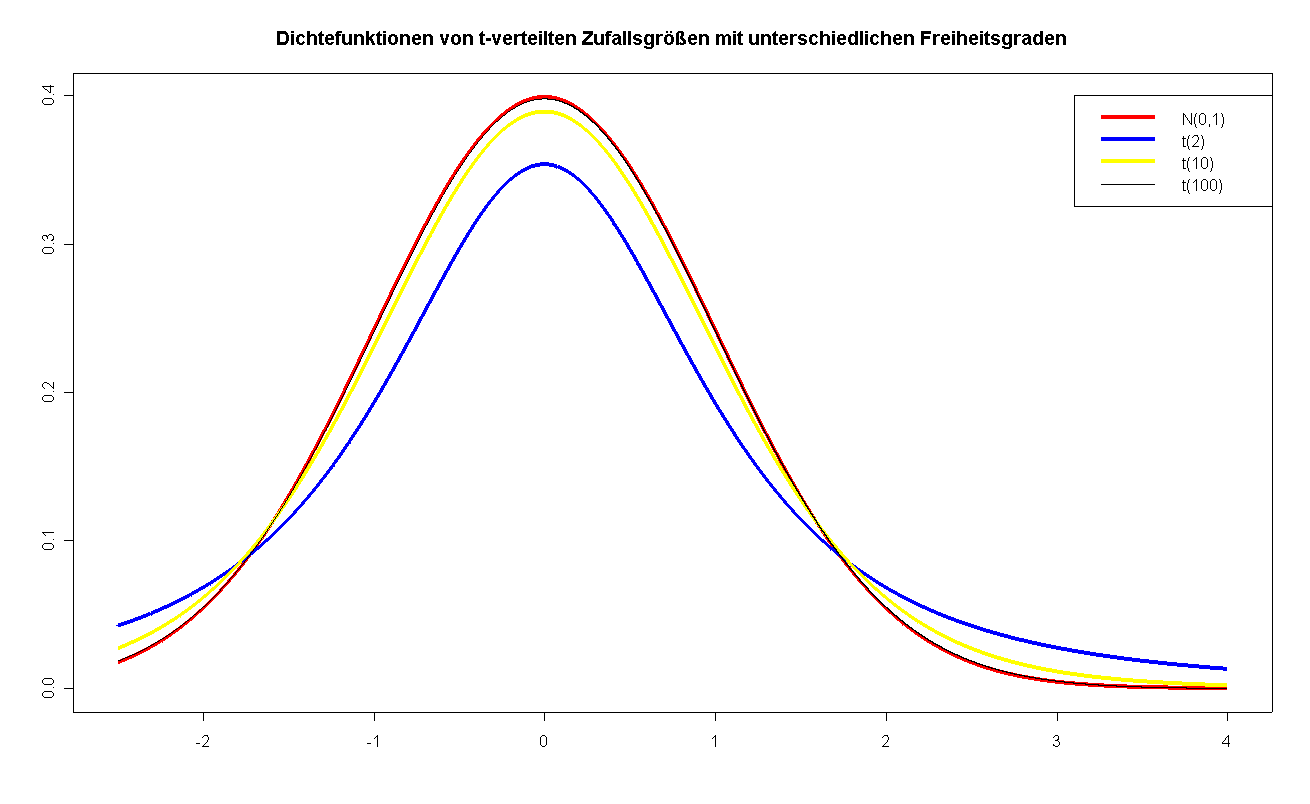
\includegraphics[width=8cm,height=4cm]{./bilder/T-Verteilung.png}\\
	$\lim\limits_{x\rightarrow \infty}$ = 0 aber langsamer wie bei Gaussverteilung 
\end{minipage}

\begin{tabular}{p{2cm}p{16cm}}
	Beispiel: & \textcolor{green}{10} Messungen ergeben Durchschnittswert
	\textcolor{red}{4{,}7} und eine Standardabweichung \textcolor{blue}{0{,}1}.
	Finde ein 99\%  Konfidenzintervall für $\mu$.\\
	
	Finde t: & \begin{tabular}{| c | c | c | c |}
		\hline
		$k=\textcolor{green}{n}-1$ & \ldots & 0{,}995\\
		\hline
		\vdots & \vdots & \vdots \\
		\hline
		9 & \ldots & 3{,}2498\\
		\hline
	\end{tabular}
	
	$\left[\textcolor{red}{\bar{X}}-3,2498\frac{\textcolor{blue}{S}}{\sqrt{\textcolor{green}{n}}},
	\textcolor{red}{\bar{X}}+3,2498\frac{\textcolor{blue}{S}}{\sqrt{\textcolor{green}{n}}}\right]
	\Rightarrow 
	\left[{\color{red}4{,}7}-3{,}2498\frac{\textcolor{blue}{0{,}1}}{\sqrt{\textcolor{green}{10}}},
	\textcolor{red}{4{,}7}+3{,}2498\frac{\textcolor{blue}{0{,}1}}{\sqrt{\textcolor{green}{10}}}\right]$\\ \\
	& $\mu\in \left[4{,}5072, 4{,}8028\right]$ mit Wahrscheinlichkeit 99\%
\end{tabular}